\section{Introduction}
	
	Despite its significance in nature, the brain is one of the least understood
	entities known to science. Current attempts to understand the brain centre on
	building models of its behaviour. Though models such as Spaun are able to
	produce high-level, realistic behaviour, they run slowly conventional
	computers taking 2.5 hours to simulate one second of neural activity
	\cite{eliasmith12}.
	
	Neural models are typically a large graph of `neurons' which are connected to
	potentially thousands of others. Signals, known as spikes, are produced and
	received between connected neurons resulting in large amounts of very small
	messages being passed between processors \cite{vainbrand11}. Because neurons
	are often cheap to simulate, typical super computers featuring powerful
	processors with comparatively limited interconnection networks perform poorly.
	
	The Blue Brain project has built a model with extremely realistic neuron
	behaviour which can exploit typical super-computer resources \cite{markram06}.
	However, models are severely limited in size to hundreds of thousands of
	neurons compared with the 85 billion in a human brain. This work instead
	focuses on the simulation of large networks of simple neurons such as Spaun.
	
	Due to the unsuitability of conventional architectures, special-purpose
	systems have been built for neural simulation. In this short report current
	attempts to overcome these limitations are described followed by an overview
	of preliminary work carried out on the SpiNNaker brain simulation
	architecture. The report concludes with the research plan proposed to develop
	this research to eventually yield an improved architecture for brain
	simulation with a focus on the topology of the interconnection network.

\section{Brain Simulators}
	
	Current special purpose brain-simulation architectures can be divided into two
	types categories: those based on conventional digital circuits and those based
	on analogue electronics inspired by the brain's analogue mechanisms. Though
	analogue systems can be very power efficient the maturity of digital design
	techniques have meant that modern analogue simulators are `mixed mode'
	implementing only the neurons using analogue electronics and interconnecting
	them with digital electronics. As a result, the interconnection networks of
	modern analogue and digital simulators are typically directly comparable.
	
	This section describes the interconnection network of three notable
	architectures. A wider and more detailed survey of current simulation
	architectures is available by Misra and Saha \cite{misra10}.
	
	\begin{figure}
		
		\center
		\begin{subfigure}[b]{0.32\textwidth}
			\center
			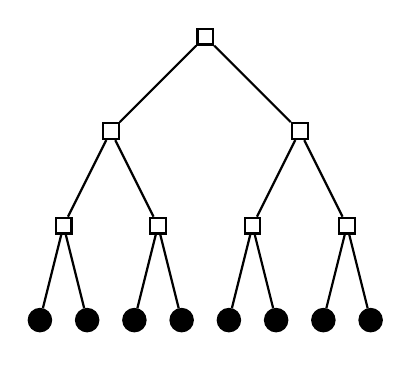
\begin{tikzpicture}[thick, node distance=1em,level distance=1.2cm]
	
	% Bodge/Hack to vertically center with mesh and torus figures.
	\draw [white] (-1.3cm,-3.85cm) rectangle ++(2cm,2cm);
	
	\begin{scope}[every node/.style={draw,rectangle,thick},             inner sep=0.1cm]
		\tikzstyle{level 1}=[sibling distance=2.4cm,every child/.style  ={},inner sep=0.1cm]
		\tikzstyle{level 2}=[sibling distance=1.2cm,every child/.style  ={},inner sep=0.1cm]
		\tikzstyle{level 3}=[sibling distance=0.6cm,every child/.style={},inner sep=0.1cm]
		
		\node {}
			child {node {}
				child {node {}
					child {node [fill,circle] {}}
					child {node [fill,circle] {}}
				}
				child {node {}
					child {node [fill,circle] {}}
					child {node [fill,circle] {}}
				}
			}
			child {node {}
				child {node {}
					child {node [fill,circle] {}}
					child {node [fill,circle] {}}
				}
				child {node {}
					child {node [fill,circle] {}}
					child {node [fill,circle] {}}
				}
			}
		;
	\end{scope}
	
\end{tikzpicture}


			\caption{Binary Tree}
			\label{fig:binary-tree}
		\end{subfigure}
		\begin{subfigure}[b]{0.32\textwidth}
			\center
			\begin{tikzpicture}[thick,inner sep=0.1cm,3d/perspective eye={0,10,20}]
	\def\width{5}
	\def\height{5}
	
	\def\tubewidth{1}
	\def\holesize{5}
	
	\pgfmathtruncatemacro{\widthh}{\width - 1}
	\pgfmathtruncatemacro{\heightt}{\height - 1}
	
	\clip (-0.7,-0.3) rectangle (\widthh+0.7,\heightt+0.7);
	
	\foreach \lx in {0,...,\widthh}{
		\foreach \ly in {0,...,\heightt}{
			\node [fill,circle]
			      (node X\lx Y\ly) at (\lx, \ly)
			      {};
		}
	}
	
	% Draw normal links
	\foreach \x in {0,...,\widthh}{
		\foreach \y in {0,...,\heightt}{
			\pgfmathtruncatemacro{\xx}{\x + 1}
			\pgfmathtruncatemacro{\yy}{\y + 1}
			\ifthenelse{\xx < \width}{
				\draw (node X\x Y\y.center) -- (node X\xx Y\y.center);
			}{
				%\draw (node X\x Y\y.center) -- (node X0Y\y.center);
			}
			\ifthenelse{\yy < \height}{
				\draw (node X\x Y\y.center) -- (node X\x Y\yy.center);
			}{
				%\draw (node X\x Y\y.center) -- (node X\x Y0.center);
			}
		}
	}
	
	% Draw Long Links
	% \begin{pgfonlayer}{background}
	% 	\foreach \x in {0,...,\widthh}{
	% 		\draw [help lines] (node X\x Y0.center)
	% 		            .. controls +(0.7,-2.0)
	% 		                    and +(0.7,2.0)
	% 		            .. (node X\x Y\heightt.center);
	% 	}
	% 	\foreach \y in {0,...,\heightt}{
	% 		\draw [help lines] (node X0Y\y.center)
	% 		            .. controls +(-2.0,0.7)
	% 		                    and +(2.0,0.7)
	% 		            .. (node X\widthh Y\y.center);
	% 	}
	% \end{pgfonlayer}
	
\end{tikzpicture}


			\caption{2D Mesh}
			\label{fig:mesh}
		\end{subfigure}
		\begin{subfigure}[b]{0.32\textwidth}
			\center
			\begin{tikzpicture}[thick,inner sep=0.1cm,3d/perspective eye={0,10,20}]
	\def\width{5}
	\def\height{5}
	
	\def\tubewidth{1}
	\def\holesize{5}
	
	\pgfmathtruncatemacro{\widthh}{\width - 1}
	\pgfmathtruncatemacro{\heightt}{\height - 1}
	
	\clip (-0.7,-0.3) rectangle (\widthh+0.7,\heightt+0.7);
	
	\foreach \lx in {0,...,\widthh}{
		\foreach \ly in {0,...,\heightt}{
			\node [fill,circle]
			      (node X\lx Y\ly) at (\lx, \ly)
			      {};
		}
	}
	
	% Draw normal links
	\foreach \x in {0,...,\widthh}{
		\foreach \y in {0,...,\heightt}{
			\pgfmathtruncatemacro{\xx}{\x + 1}
			\pgfmathtruncatemacro{\yy}{\y + 1}
			\ifthenelse{\xx < \width}{
				\draw (node X\x Y\y.center) -- (node X\xx Y\y.center);
			}{
				%\draw (node X\x Y\y.center) -- (node X0Y\y.center);
			}
			\ifthenelse{\yy < \height}{
				\draw (node X\x Y\y.center) -- (node X\x Y\yy.center);
			}{
				%\draw (node X\x Y\y.center) -- (node X\x Y0.center);
			}
		}
	}
	
	% Draw Long Links
	\begin{pgfonlayer}{background}
		\foreach \x in {0,...,\widthh}{
			\draw  (node X\x Y0.center)
			            .. controls +(0.5,-1.8)
			                    and +(0.5,1.8)
			            .. (node X\x Y\heightt.center);
		}
		\foreach \y in {0,...,\heightt}{
			\draw  (node X0Y\y.center)
			            .. controls +(-1.8,0.5)
			                    and +(1.8,0.5)
			            .. (node X\widthh Y\y.center);
		}
	\end{pgfonlayer}
	
\end{tikzpicture}


			\caption{2D Torus}
			\label{fig:torus}
		\end{subfigure}
		
		\caption{Network topology examples. Dots represent chips, boxes represent
		switches which forward messages but perform no other computation.}
		\label{fig:network-topology-examples}
		
	\end{figure}
	
	\subsection{Neurogrid}
		
		The Neurogrid architecture consists of chips with analogue hardware to
		simulate tens of thousands of neurons. Spikes from these neurons are output
		by the chip one at a time (serially) and must be routed to each of the
		target neurons which may reside in other chips. Current prototypes feature
		16 chips which form the leaves of a binary tree (figure
		\ref{fig:binary-tree}). This architecture can simulate around a million
		neurons with 100,000 times less power than a conventional super-computer
		\cite{choudhary12}.
		
		The binary tree interconnection network topology is scalable with network
		latency, in the ideal case, increasing $O(\log{N})$ with the number of
		chips. For neural simulation, however, tree topologies have been shown by
		Vainbrand and Ginosar to be non-optimal requiring large amounts of hardware
		to achieve the bandwidth required to transmit large numbers of spikes
		between nodes \cite{vainbrand11}.
	
	\subsection{BrainScaleS}
	
		The BrainScaleS project has developed an architecture unconventionally uses
		an entire silicon wafer on which tens of chips have been produced
		side-by-side. Each chip contains a number of analogue neuron simulators
		which are interconnected via a 2D mesh network (figure \ref{fig:mesh}).
		Spikes can be forwarded from chip to chip until they reach their destination
		\cite{schemmel08}. It is intended that multiple wafers will be combined with
		conventional Internet Protocol (IP) switches.
		
		Though mesh networks are easily scaled in principle, the BrainScaleS
		architecture is limited by the maximum size of a silicon wafer. The topology
		to be used to connect wafers together has not yet been decided though since
		silicon wafers are circular, the mesh topology cannot be cleanly tessellated
		with further wafers detracting from the performance of the network.
	
	\subsection{SpiNNaker}
	
		Finally, the focus of my work so far: SpiNNaker has many small processors
		connected via a torus network whose size is only limited by the address
		space available to neurons. Network optimised for small (maybe zero-data)
		packets.  Unlike the first two it runs simulations in software making it far
		more flexible, easier with current understanding of electronics but less
		power efficient.
		
		Here's how it looks in implemented hardware: cores, chips and boards.

\section{Preliminary Work}

Current work has focused on SpiNNaker and possible extensions to it.

\subsection{SpiNNaker Topology}

To make things practical, board-to-board links use different technology to
within-board links as hundreds of wires is impractical between boards but fine
on-board. Built a simulator which simulates a model of the network to examine
how these links affect performance. Found that these links do introduce a
significant penalty but one which is probably not an issue for current
simulation needs but may be later when latency becomes more sensitive.

\subsection{SpiNNaker Wiring}

Wiring up big machines is tough. Boards must be placed into cabinets and wires
run by hand between them. Three major constraints: cost of the cables, length to
allow tech to work fast and complexity to make it possible to wire up by hand.
Work was done to propose wiring schemes for large SpiNNaker machines of 1,200
boards.

Cost constraint solved by using the high speed links tested previously.

In SpiNNaker you have a torus meaning you get links which span one end of the
system to another. This violates the length requirement. To solve this the
system is 'folded'. This is illustrated in a ring network (figure) and easily
generalises to a torus. This removes the long wrap-around link eliminating long
wires from the system.

A folded system, when mapped into cabinets and racks, becomes very non-uniform.
Luckily it isn't as bad as it looks, especially for larger systems (see figure
of full machine) but listing every connection and expecting a human to do it
isn't viable. Regularity can be found by dividing the connections up by logical
direction and whether they leave the cabinet they're in or not. For a large
machine the number of instructions therefore drops from 3,600 (one per
connection) to 53 (with each rule being used to connect hundreds of wires).

\subsection{Small-World Super-Computers}

The connections in the brain, along with many graphs observed in nature exhibits
the 'small world' property, first described by Frigyes Karinthy in 1929, which
states that the maximum length of a path between any two nodes in a small-world
graph is very short. This idea is popularly known as the theory of six degrees
of seperation and is the basis of theoretical work carried out by Watts and
Strogatz who proposed an algorithm for generating random graphs with the
small-world property.

This work extends this model to generate torus-like networks (as in SpiNNaker)
augmented with random connections and found that an great reduction in the
number of links messages must traverse in the network was achieved for a modest
increase in the number of connections in the network.

Based on the work on wiring practicality, this system was extended to generate
networks which met the wiring practicality criteria outlined above. Despite
severe restrictions on allowed connections the new topology still resulted in
improved performance.

\section{Research Plan}

[Gantt Chart]

Initial work will focus on the development of a simulator for SpiNNaker's
interconnect topology to contribute to work comparing actual prototype SpiNNaker
hardware against various software models of its behaviour. This work is hoped
for Journal publication later this year. This work is expected to take 

With the development of a suitable simulator, this will be extended to perform
more detailed experiments on the semi-random small-world networks examined in
the preliminary work.

With the process for extending the simulator and performing comparisons proven
for the small-world network case, other less conventional topologies such as
express cubes, which offer latency advantages over standard torus networks will
be examined and compared.

Work will continue looking at the impact of 'place and route', the task of
allocating parts of a neural simulation to spinnaker's processor resources and
routing spikes between them. This will provide a further comparison to be drawn
between the topologies examined as place and route can be extremely
computationally expensive. In addition, this will consider the effect of
multicast traffic.

The penultimate stage of the project will be to compare available link
technologies. The tech used in SpiNNaker is no longer available and a
replacement is needed.

The final goal of the project will be to bring together the work to suggest a
new architecture for a next-generation SpiNNaker.

